\newpage
\setcounter{figure}{0}

\section{Pregled korištenih tehnologija i algoritama} % (fold)
\label{sec:Tehnologija i teorija}

\subsection{Microsof Kinect 3D kamera} % (fold)
\label{sub:Microsof Kinect 3D kamera}

Kinect je RGB-D senzor koji daje sliku u boji sinkroniziranu s dubinskom
slikom. Inicijalno je korišten kao ulazni uređaj za Microsoft Xbox
igračku konzolu. Algoritmima za prepoznavanje ljudskih pokreta omogućava
interakciju između igre i igrača bez potrebe za korištenjem kontrolera.
Nakon pojave senzora zajednica znanstvenika koji proučavaju računalni
vidi otkrila je da tehnologija korištena za dohvaćanje dubine može biti
upotrebljena za puno više od igranja za puno manje cijenu nego
tradicionalne 3D kamere kao što su stereo i Time-of-flight kamere.

Dodatno, komplementarna priroda informacije o dubini na slici koju pruža
Kinect, olakšava nova potencijalna rješenja klasičnih problema računalnog
vida. U samo dvije godine nakon puštanja u prodaju Kinecta, velik broj
znanstvenih članaka i demonstracija se pojavio na raznim konferencijama.

\begin{figure}[h]
\centering
\includegraphics[scale=0.15]{figures/kinect.png}
\caption{Shematski prikaz Kinect kamere, izvor:~\cite{HanSXS13}}
\label{fig:kinect.png}
\end{figure}

\subsubsection{Tehničke specifikacije} % (fold)
\label{ssub:Tehničke specifikacije}

Slika~\ref{fig:kinect.png} prikazuje raspored Kinect senzora. Kinect se
sastoji od infracrevnog (IR) projektora, IR kamere i RGB kamere.
Dubinski senzor se sastoji od IR projektora i IR kamere. IR projektor
projicira IR uzorak točkastih mrlja na 3D scenu dok IR kamera hvata
reflektirane IR mrlje. Kinect radi na principu strukturirane svjetlosti.
Geometrijska veza između IR projektora i IR kamere se ostvaruje offline
kalibracijskom procedurom. IR projektor projicira poznat uzorak
svjetlosnih mrlja na scenu. IR svjetlost je nevidljiva RGB kameri ali
je vidljiva IR kameri. Kako je svaki lokalni uzorak projiciranih točaka
jedinstven, spajanje promatranih lokalnih uzoraka točaka sa slike
s kalibriranim projektorovim uzorkom točaka je ostvarivo. Više o
principu strukturirane svjetlosti u~\cite{structured:light}.\\

\newpage
Tehničke informacije o kameri:
\begin{itemize}
    \item \textbf{RGB kamera} daje sliku rezolucije \(640\times480\)
        piksela pri osvježavanju slike od 30Hz. Postoji i opcija davanja
        slike rezolucije \(1280 \times 1024\) piksela ali se dobije samo 10
        sličica po sekundi.
    \item \textbf{3D Dubinski senzor} se sastoji od IR laserskog
        projektora i IR kamere. Zajedno, projektor i kamera kreiraju
        dubinsku mapu, koja pruža informaciju o udaljenosti između
        objekta i kamere. Senzor ima praktično ograničenje u dometu 
        0.8m - 3.5m. Kamera daje video od 30 sličica po sekundi s
        rezolucijom \(640 \times 480\) piksela. Vidno polje senzora je
        \(57\,^{\circ}\) horizontalno i \(43\,^{\circ}\) vertikalno.
    \item \textbf{Motorni nagib} upravlja nagibom Kinecta. Nagib može
        biti pomaknuti \(27\,^{\circ}\) gore ili dolje.
\end{itemize}

% subsubsection Tehničke specifikacije (end)

% subsection Microsof Kinect 3D kamera (end)

\newpage
\subsection{ROS biblioteka i alati} % (fold)
\label{sub:ROS biblioteka i alati}

ROS~\cite{ros} (engl. \textit{Robot Operating System}) je set programskih
biblioteka i alata koji pomažu programerima kreirati aplikacije za
robote. Pruža hardversku abstrakciju, upravljačke programe, biblioteke,
vizualizaciju, komunikaciju, upravljanje paketima i dr. ROS je
licenciran BSD licencom, koja spada pod licence otvorenog koda.

\begin{figure}[h]
\centering
\includegraphics[scale=0.45]{figures/ros.png}
\caption{Shematski prikaz ROSa}
\label{fig:ros.png}
\end{figure}

U ovom radu ROS se dotiče kroz program RGBDSlam koji je opisan u
potpoglavlju~\ref{sub:Snimanje scene 3D kamerom i RGBDSlam programom} te se oslanja na
njegove biblioteke, upravljačke programe i alate. Tako RGBDSlam koristi
OpenNI upravljački program za komunikaciju s Kinect kamerom u obliku ros
programskog paketa (\texttt{ros-fuerte-openni-launch}). Također, RGBDSlam
koristi i niz drugih paketa iz ROS biblioteke~\cite{web:rgbdslam}

% subsection ROS biblioteka i alati (end)

\newpage
\subsection{Biblioteka Pointcloud} % (fold)
\label{sub:Biblioteka Pointcloud}

PCL~\cite{pcl} (engl. \textit{Point Cloud Library}
slika~\ref{fig:pcl.png}) je otvoren projekt za procesiranje 2D/3D slika
i oblaka točaka. PCL biblioteka sadržava niz najsuvremenijih algoritama
za filtriranje, estimaciju značajki, rekonstrukciju površina,
registraciju, uklapanje modela i segmentaciju.  Ti algoritmi se mogu
koristiti za: izbacivanje odudarajućih vrijednosti iz šumovith
podataka, spajanje 3D oblaka točaka, segementiranje relevantnih dijelova
scene, izvlačenje ključnih točaka i računanje deskriptora za
prepoznavanje objekata na temelju njihove geometrije, kreiranje i
prikazivanje površina iz oblaka točaka itd.

\begin{figure}[h]
\centering
\includegraphics[scale=0.15]{figures/pcl.png}
\caption{PCL logo}
\label{fig:pcl.png}
\end{figure}

PCL je objavljen pod BSD licencom i softver je otvorenog koda. Što znači
da je slobodan za upotrebu u komercijalne i akademske svrhe.

PCL se uspješno prevodi na GNU/Linux, MacOS, Windows i Android/iOS
platformama. Zbog olakšanog razvijanja podijeljen je na više manjh
biblioteka koje se mogu prevoditi zasebno. PCL se može prikazati kao
graf biblioteka kao što je prikazano na slici~\ref{fig:pcl-graph.png}

\setcounter{figure}{0}
\begin{figure}[h]
\renewcommand{\figurename}{Grafikon}
\centering
\includegraphics[scale=0.40]{figures/pcl-graph.png}
\caption{Graf PCL biblioteka}
\label{fig:pcl-graph.png}
\end{figure}

% subsection Biblioteka Pointcloud (end)


\newpage
\subsection{Istovremena lokalizacija i mapiranje} % (fold)
\label{sub:Slam}
Jedno od najznačajnijih područja istraživanja na polju mobilne robotike
su metode istovremene lokalizacije i mapiranja
(engl.\textit{Simultaneous Localization and Mapping} - SLAM). SLAM su
originalno razvili Hugh Durrant-Whyte i John J.
Leonard~\cite{Durrant:91b} koji su rad bazirali na prethodnom radu
Smitha, Selfa and Cheesemana~\cite{Smith86}. SLAM se bavi rješavanjem
problema izgradnje mape nepoznate okoline mobilnog robota te istovremeno
navigiranje robota okolinom koristeći tu mapu.

SLAM se sastoji iz nekoliko koraka: izvlačenja orijentira, pridruživanja
podataka, estimiranja stanja, ažuriranja stanja i ažuriranja orijentira.
Postoji više načina kako realizirati svaki od tih koraka. SLAM se može
primjeniti na 2D i 3D kretanje.

\subsubsection{Osnovna ideja i kratak pregled koraka} % (fold)
\label{ssub:Osnovna ideja }
Proces istovremene lokalizacije i mapiranja se sastoji iz nekoliko
koraka. Cilj procesa je koristiti precepciju okolinu za ažuriranje pozicije robota.
Zbog nesavršenosti odometrije robota nije dobro osloniti se samo na nju
kako bi se pronašla pozicija robota već se može koristiti lasersko
skeniranje okoline ili, kao u slučaju RGBDSlam programa, Kinect 3D kamera
kako bi pronašli pravu poziciju robota/kamere. To se postiže
detekcijom značajki u okolini i promatranjem tih značajki kada se
robot pomakne. EKF (\textit{Extended Kalman Filter}) prošireni Kalmanov
filter je jezgra SLAM procesa. EKF je odgovoran za ažuriranje pozicije
na kojoj robot ``misli'' da se nalazi koristeći izvučene značajke. Takve
značajke se još nazivaju i orijentiri. EKF prati estimaciju nesigurnosti
pozicije robota i nesigurnosti orijentira iz okoline. Pregled SLAM
procesa~\footnotemark[1] se nalazi na grafikonu~\ref{fig:slam-overview.pdf}  

\footnotetext[1]{%
Grafikon je inspiriran sličnim grafikonom iz rada SLAM for
Dummies~\cite{web:slam} }

\begin{figure}[h]
\renewcommand{\figurename}{Grafikon}
\centering
\includegraphics[scale=0.4]{figures/slam-overview.pdf}
\caption{Pregled SLAM procesa}
\label{fig:slam-overview.pdf}
\end{figure}

Kad se odometrija promijeni zato što se robot pomakao, nesigurnost koja se
tiče robotove nove pozicije se ažurira u EKF koristeći ažuriranje
odometrije. Orijentiri se tada detektiraju u okoline iz robotove nove
pozicije. Robot tada pokušava asocirati detektirane orijentire s prije zapaženim
orijentirima spremljenim u kratu. Ponovno zapaženi orijentiri se tada koriste za ažuriranje
pozicije robota u EKFu. Orijentiri koji prije nisu zapaženi se dodaju u
kartu kako bih se mogli koristiti kasnije. U svakom od opisanih koraka EKF
računa estimaciju robotove trenutne pozicije. 

\newpage
\subsubsection{Proširen Kalmanov filter - EKF} % (fold)
\label{ssub:Proširen Kalmanov filter - EKF}

Kalmanov filter je algoritam koji koristi niz mjerenja pribavljenih
tijekom vremena, koja sadržavaju šum i ostale netočnosti, te računa
estimacije nepoznatih varijabli koje su, u slučaju zadovoljenja
pretpostavki algoritma, preciznije od računa baziranom samo na jednom
mjerenju. Konkretnije, Kalmanov filter se izvršava rekurzivno na nizu
šumovith ulaznih podataka i računa statistički optimalnu estimaciju
sustava stanja. Filter je nazvan po Rudolfu E. Kalmanu~\cite{Kalman}
koji je jedan od primarnih razvijatelja teorije.


Algoritam je podijeljen u dva koraka kao što se vidi na
grafikonu~\ref{fig:basic-kalman}. U prvom predikcijskom koraku Kalmanov
filter računa estimaciju trenutnih varijabla stanja s njihovim
nesigurnostima na temelju modela kretanja robota. U drugom korekcijskom
koraku, kada je promotren rezultat sljedećeg mjerenja (koje isto ima
greške pri mjerenju i šum mjerenja), izračunata estimacija se korigira
upotrebom težinske sredine gdje se više težine daje estimaciji s većom
vjerojatnošću.

\begin{figure}[H]
\centering
\renewcommand{\figurename}{Grafikon}
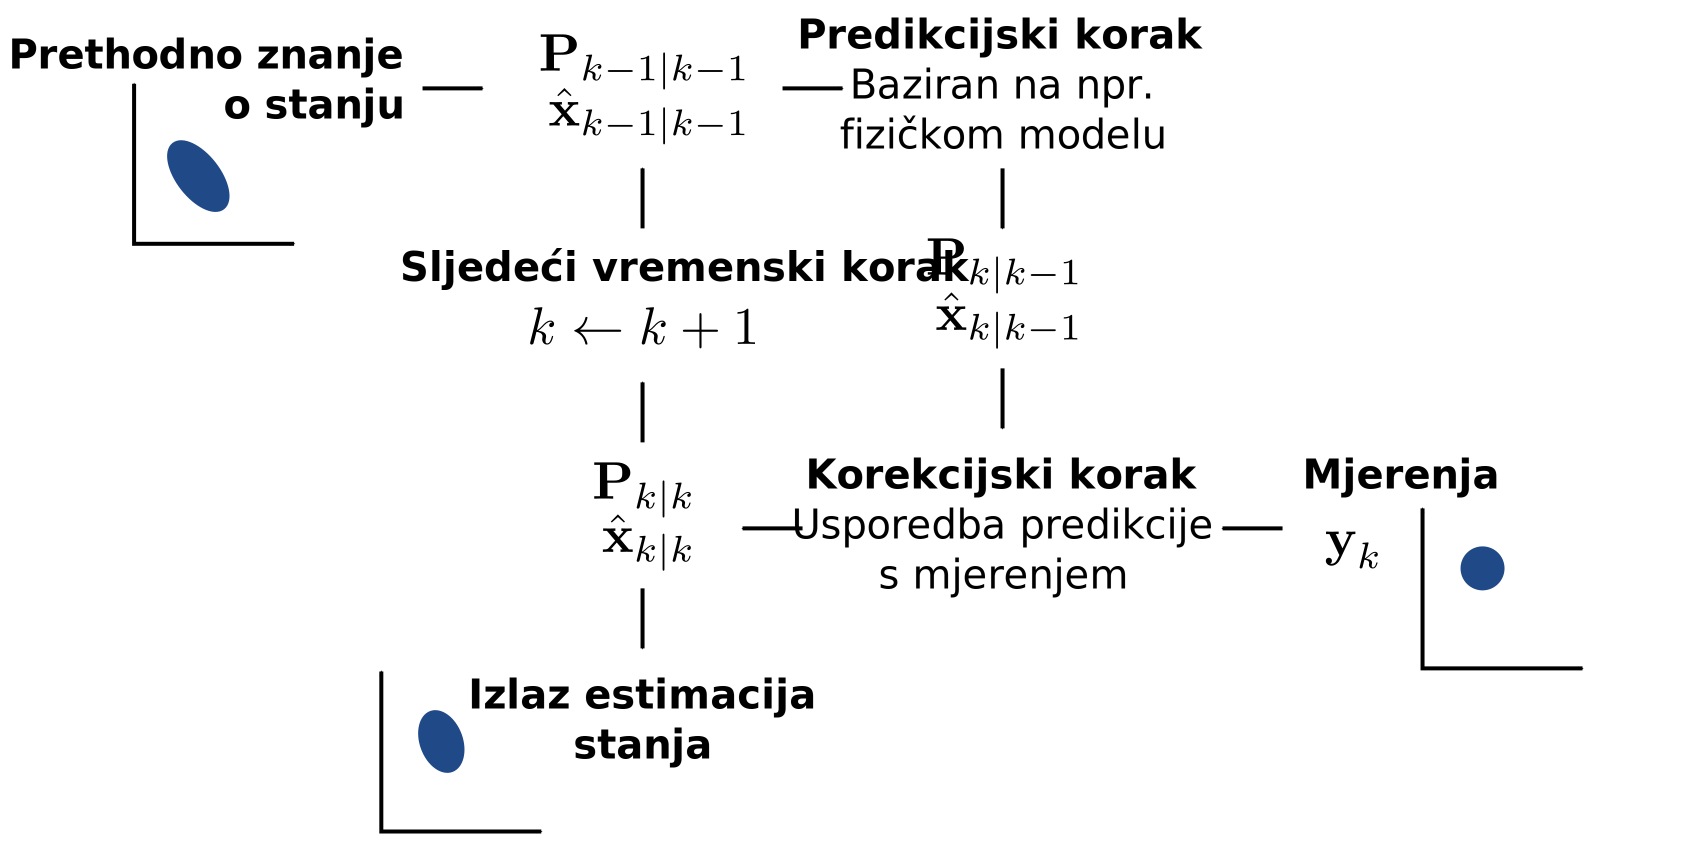
\includegraphics[scale=0.35]{figures/basic-kalman.pdf}
\caption{Osnova Kalmanovog filtra}
\label{fig:basic-kalman}
\end{figure}

\textbf{Prošireni Kalmanov filter} je nelinearna verzija Kalmanovog
filtra gdje promjena stanja i promatrani model ne moraju biti linearne
funkcije.

% subsubsection Proširen Kalmanov filter - EKF (end)

% subsubsection Osnovna ideja  (end)
% subsection Slam (end)

\newpage
\subsection{Poisson algoritam za rekonstrukciju površine} % (fold)
\label{sub:Poisson}
Poisson algoritam za rekonstrukciju površine~\cite{Kazhdan:2006}
razvijen je suradnjom Michaela Kazhdana i Matthewa Bolitha s Johns
Hopkins sveučilišta u Baltimoru i Huguesa Hoppea iz Microsoft Researcha
u Redmondu. Također Kazhdan i Bolitho su implementirali\footnotemark[1]
Poisson algoritam i objavili kod pod BSD licencom. Na osnovu tog rada
algoritam je dodan i u PCL biblioteku.

U ovom potpoglavlju nalazi se osnovna ideja i kratak matematički pregled
algoritma. Opisano je ograničenje algoritma te parametri kojima se može
upravljati rekonstrukcijom površine.

\footnotetext[1]{%
Originalna implementacija Poisson algoritma se nalazi na 
\url{http://www.cs.jhu.edu/~misha/Code/PoissonRecon/Version5.5/}}

% Rekonstrukcija 3D površina iz uzorka točaka je dobro proučavan problem u
% računalnoj grafici. Ona omogućava uklapanje skeniranih
% podataka, ispunjavanje površinskih rupa i ponovnu izgradnju postojećih
% modela.

\subsubsection{Osnovna ideja i kratak matematički pregled} % (fold)
\label{ssub:Osnovna ideja i kratak matematički pregled}

Poisson algoritam pristupa problemu rekonstrukcije površine rješavanjem
Poissonove jednadžbe. To čini upotrebom metode implicitne funkcije.
Točnije računanjem 3D indikacijske funkcije \(\chi\) definirane s 1 u
točkama unutar modela, odnosno s 0 u točkama izvan i dohvaćanjem
rekonstruktruirane površine izvlačenjem odgovarajuće izopovršine.

Algoritam se oslanja na ideju da postoji cjelovita veza između
orijentiranih normala uzetih s površine modela i indikacijske funkcije
modela. Točnije, gradijent indikacijske funkcije je polje vektora koje
je uglavnom popunjeno nulama (jer je indikacijska funkcija uglavnom
konstantna), osim kod točaka blizu površine gdje je jednako unutrašnjim
normalama površine. Stoga, uzorci orijentiranih normala mogu biti
promatrani kao gradijent modela indikacijske funkcije kao što je
prikazano na slici~\ref{fig:poisson-reconstruction.png}

\begin{figure}[h]
\centering
\includegraphics[scale=0.35]{figures/poisson-reconstruction.png}
\caption[]{Prikaz Poisson rekonstrukcije u 2D,
    izvor:~\cite{Kazhdan:2006}}
\label{fig:poisson-reconstruction.png}
\end{figure}

Problem računanja indikacijske funkcije se svodi na invertiranje
operatora gradijenta, odnosno pronalazak funkcije skalara \(\chi\) čiji
gradijent najbolje aproksimira polje vektora \(\vec{V}\) definirano
uzorcima, odnosno 

\begin{equation*}
min_\chi \|\nabla\chi - \vec{V}\|.
\end{equation*}

Ako se primjeni operator divergencije, tada se taj problem pretvara u
standardni Poissonov problem: računanje funkcije skalara \(\chi\) čiji
laplasijan (divergencija gradijenta) je jednak divergenciji polja
vektora \(\vec{V}\),

\begin{equation*}
\Delta \chi \equiv \nabla \cdot \nabla\chi = \nabla \cdot \vec{V}.
\end{equation*}

Predstavljanje rekonstrukciju površine kao Poissonov problem pruža
nekoliko prednosti. Mnoge implicitne metode uklapanja površina
segementiraju podatke u regije za lokalno uklapanje i onda te lokalne
aproksimacije spajaju upotrebom funkcija stapanja. Za razliku od njih,
Poisson rekonstrukcija je globalno rješenje koje razmatra sve podatke
odjednom, bez upotrebe heurstičkih podijela i stapanja. Zbog toga
Poisson rekonstrukcija kreira izrazito glatku površinu koja robusno
aproksimira šumovite podatke.  

Za izvlačenje izopovršine Poisson algoritam koristi Marching Cubes
algoritam~\cite{Lorensen87marchingcubes} koji kreira octree strukturu
podataka za prikaz površine.  Kao što se vidi na
slici~\ref{fig:poisson-marching-cubes.png} Marching Cubes algoritam
dijeli oblak točaka u mrežu voxela marširajući kroz oblak i analizira
koje točke čine izopovršinu objekta.  Detektiranjem koji rubovi voxela
presjecaju izopovršinu modela algoritam kreira mrežu trokuta. Više
informacija o izvlačenju površine se mogu pronaći u radu “Unconstrained
Isosurface Extraction on Arbitrary Octrees” Michaela
Kahzdana~\cite{Kazhdan:2007}

\begin{figure}[h]
\centering
\includegraphics[scale=0.8]{figures/poisson-marching-cubes.png}
\caption[]{Prikaz Marching cubes algoritma, izvor:~\cite{Kazhdan:2007}}
\label{fig:poisson-marching-cubes.png}
\end{figure}

% subsubsection Osnovna ideja i kratak matematički pregled (end)

\subsubsection{Ograničenje Poisson algoritma} % (fold)
\label{ssub:Ograničenje Poisson algoritma}

Ograničenje implementacije Poisson algoritma je u tome što ne uzima u
obzir informacije vezane uz način snimanja oblaka točaka.
Slika~\ref{fig:poisson-buddha.png} pokazuje kip Bude i vidi se primjer takvog
ograničenja. Budući da nema točaka između Budinih nogu, Poisson
algoritam spaja te dvije regije. Algoritam se može unaprijediti
ugradnjom dodatne informacije poput vidokruga i na taj način izbjeći to
ograničenje.


\begin{figure}[h]
\centering
\includegraphics[scale=0.20]{figures/poisson-buddha.png}
\caption[]{Rekonstrukcija modela ``Happy Buddha'' 
VRIP\footnotemark[2] algoritam (lijevo) i Poisson algoritma (desno),
izvor:~\cite{Kazhdan:2006}}
\label{fig:poisson-buddha.png}
\end{figure}

\footnotetext[2]{%
VRIP - Volumetric Range Image Processing~\cite{Curless:1996VRIP}}

% subsubsection Ograničenje Poisson algoritma (end)

\newpage
\subsubsection{Parametri Poisson algoritma} % (fold)
\label{ssub:Parametri Poisson algoritma}
Postoji nekoliko parametara koji utječu na rezultat rekonstrukcije.
\begin{itemize}
    \item \texttt{Depth:} dubina octree stabla koje se koristi za
        rekonstrukciju. Pretpostavljena vrijednost 8.
    \item \texttt{SolverDivide:} postavlja dubinu kod kojeg bloka
        Gauss-Seidel metoda riješava Laplaceovu jednadžbu. Pretpostavljena
        vrijednost 8.
    \item \texttt{IsoDivide:} postavlja dubinu kod kojeg bloka
        ekstraktor izopovršine izvlači izopovršinu. Pretpostavljena vrijednost
        8.
    \item \texttt{SamplesPerNode:} postavlja minimalni broj točaka koje
        se trebaju nalaziti unutar octree čvora kako se octree
        konstrukcija prilagođava gustoći uzorkovanja. Za podatke bez
        šuma 1 - 5, sa šumom 15 - 20. Pretpostavljena vrijednost 1.
    \item \texttt{Scale:} omjer između promjera kocke korištne za
        rekonstrukciju i promjera kocke koja omeđuje uzorke. Pretpostavljena
        vrijednost 1.25.
    \item \texttt{Confidence:} postavljanje zastavice govori
        rekonstrukciji da koristi veličinu normala kao informaciju o
        pouzdanosti. Ako nije postavljena sve normale se normaliziraju
        prije rekonstrukcije.
\end{itemize}

Od nabrojanih parametara najvažniji utjecaj na generiranu mrežu imaju
\texttt{SamplesPerNode} i \texttt{Depth}. Veća dubina octree stabla
rezultira većom precinosti mreže voxela jer Marching Cubes algoritam
ulazi dublje u stablo. Manja dubina (između 5 i 7) daje glađi model ali
s manje detalja. \texttt{SamplesPerNode} parametar definira koliko će
točaka Marchin Cubes algoritma staviti u jedan čvor rezultantnog octree
stabla. Ako algoritam radi s podacima punim šuma velik uzorak točaka (15
- 20) po čvoru pruža glađenje ali se gube detalji. Dok rad s malim
vrijednostima (1 - 5) održava razinu detalja visokom. Velike vrijednosti
reduciraju kranji broj vrhova poligona, dok male održavaju broj vrhova
visokim.

% subsubsection Parametri Poisson algoritma (end)

% subsection Poisson (end)

% section Tehnologija i teorija (end)
